Por otro lado, para agregar un nuevo agente, es necesario presionar sobre el botón en la parte superior que es quien nos manda al método mostrado en la figura \ref{image:add1}, el cual se encarga de abrir una pequeña ventana como la de la figura \ref{image:addP}, y en este, se manda a llamar a otros 2 métodos mostrados a continuación.
\FloatBarrier
\begin{figure}[htbp!]
		\centering
	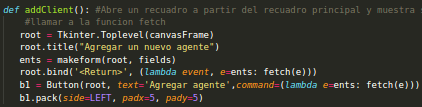
\includegraphics[width=.8 \textwidth]{images/add1}
		\caption{Método addClient.}		\label{image:add1}
\end{figure}
\FloatBarrier

\FloatBarrier
\begin{figure}[htbp!]
		\centering
	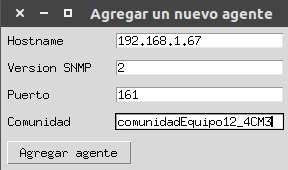
\includegraphics[width=.4 \textwidth]{images/addP}
		\caption{Pantalla desplegada para añadir un cliente nuevo.}		\label{image:addP}
\end{figure}
\FloatBarrier

Por un lado se llama al método al método mostrado en la figura \ref{image:add2}, el cual únicamente se encarga de posicionar adecuadamente los labels dentro de la ventana.
\FloatBarrier
\begin{figure}[htbp!]
		\centering
	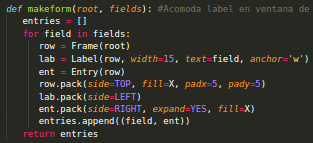
\includegraphics[width=.5 \textwidth]{images/add2}
		\caption{Método makeform.}		\label{image:add2}
\end{figure}
\FloatBarrier

Y por otro lado se lama al método fetch mostrado en la figura \ref{image:add3}, el cual obtiene todos los valores que el usuario ha agregado en los labels para registrar un agente nuevo y los agrega en una nueva línea en el archivo hosts.txt, en caso de que el archivo no exista, se crea uno nuevo. Y de igual manera, nos muestra una pequeña alerta como la de la figura \ref{image:alerta} para dar a conocer que nuestro agente ha sido creado correctamente.
\FloatBarrier
\begin{figure}[htbp!]
		\centering
	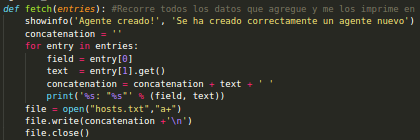
\includegraphics[width=.6 \textwidth]{images/add3}
		\caption{Pantalla desplegada para añadir un cliente nuevo.}		\label{image:add3}
\end{figure}
\FloatBarrier

\FloatBarrier
\begin{figure}[htbp!]
		\centering
	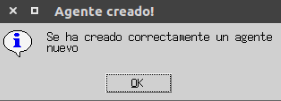
\includegraphics[width=.4 \textwidth]{images/addAlerta}
		\caption{Alerta desplegada al crearse un nuevo agente.}		\label{image:alerta}
\end{figure}
\FloatBarrier

Y se puede observar tanto en la pantalla principal(figura \ref{image:pantalla}) como en nuestro archivo de hosts (figura \ref{image:agenteAgregado}) que nuestro nuevo agente ha sido agregado correctamente.

\FloatBarrier
\begin{figure}[htbp!]
		\centering
	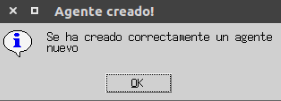
\includegraphics[width=.4 \textwidth]{images/addAlerta}
		\caption{Alerta desplegada al crearse un nuevo agente.}		\label{image:alerta}
\end{figure}
\FloatBarrier

\FloatBarrier
\begin{figure}[htbp!]
		\centering
	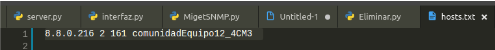
\includegraphics[width=.4 \textwidth]{images/agenteAgregado}
		\caption{Agente agregado en archivo hosts.}		\label{image:agenteAgregado}
\end{figure}
\FloatBarrier

Es importante recalcar que en la última línea del método getHostInfo mostrado en la imagen \ref{image:principal1}, se realizar un autollamado al mismo método cada 3 segundos, lo cual permite que al añadir un nuevo agente, solo se debe esperar 30 segundos para que este aparezca en la pantalla de inicio.